\chapter{Krzywe, długość i prostowalność}
\label{ma2:ch:rectifiable-curves}

Pracujemy w przestrzeni euklidesowej $\R^n$, gdzie
$n\ge1$ jest liczbą naturalną. W całym rozdziale
$a,b\in\R$ i $a<b$, o ile nie rozważamy wprost
zdegenerowanego przedziału jednopunktowego.
Przez krzywą parametryczną rozumiemy w tym rozdziale
ciągłe odwzorowanie $\gamma:[a,b]\to\R^n$.
Odróżniamy je od jego obrazu $\gamma([a,b])$. Długość drogi może
uwzględniać wielokrotne przejścia przez tę samą
część obrazu. Przygotujemy całki krzywoliniowe
z wykorzystaniem miar $\lambda_1$ i $\mathcal H^1$.

\section{Intuicja: droga, obraz i długość}

Krzywa parametryczna jest modelem ruchu:
$t$ wskazuje chwilę, a $\gamma(t)$ położenie.
Nie musi to być czas fizyczny. Zmieniając
parametryzację, można przyspieszać, zwalniać
lub zatrzymywać się, nie zmieniając długości
przebytej drogi, jeżeli zachowujemy kolejność
przejścia (lub odwracamy ją w całości).
Ścisłe uzasadnienie podamy w twierdzeniu
\ref{ma2:thm:curve-reparam}.

\paragraph{Od przemieszczenia do długości.}
Różnica $\gamma(b)-\gamma(a)$ opisuje
przemieszczenie, a jej norma jest odległością
punktów końcowych. Długość drogi może być
większa: uwzględnia wszystkie zmiany położenia,
także ruch powrotny. Gdy obserwujemy krzywą
tylko w chwilach $t_0,\ldots,t_m$, zastępujemy
ją łamaną łączącą obserwowane punkty.
Suma długości jej odcinków to
\[
 \sum_{j=1}^m
 \|\gamma(t_j)-\gamma(t_{j-1})\|_2.
\]
Dodanie chwili obserwacji nie zmniejsza
tej sumy, na mocy nierówności trójkąta.
Supremum po wszystkich skończonych
podziałach daje długość drogi.
Dla krzywej ciągłej wystarczy dowolny
ciąg podziałów o średnicach dążących
do zera (stwierdzenie
\ref{ma2:prop:curve-polygon-limit}).
Jeśli supremum jest nieskończone,
krzywa nie jest prostowalna, nawet
gdy jej obraz jest zwarty.

\begin{przyklad}[Okrąg i łamane wpisane]
\label{ma2:ex:curve-circle-polygons}
Dla $\gamma(t)=R(\cos t,\sin t)$,
$t\in[0,2\pi]$, $R>0$, rozpatrzmy
podział na $m\ge2$ równych przedziałów.
Kolejne wierzchołki dzieli kąt $2\pi/m$,
więc z tożsamości trygonometrycznych
każda cięciwa ma długość $2R\sin(\pi/m)$:
kwadrat odległości dwóch kolejnych punktów
wynosi $2R^2(1-\cos(2\pi/m))=4R^2\sin^2(\pi/m)$.
Długość łamanej wynosi
\[
 L_m=2mR\sin(\pi/m).
\]
Ponieważ $\sin u/u\to1$ przy $u\to0$,
mamy $L_m\to2\pi R$. Na mocy
\ref{ma2:prop:curve-polygon-limit}
jest to dokładna długość okręgu,
bez stosowania wzoru całkowego
z pochodną. Dla $m=2$ łamana biegnie
po tej samej średnicy w obie strony.
Dla $m=2^j$, $j\ge1$, podziały są zagnieżdżone,
a długości łamanych niemalejące.
\end{przyklad}

\begin{figure}[htbp]
\centering
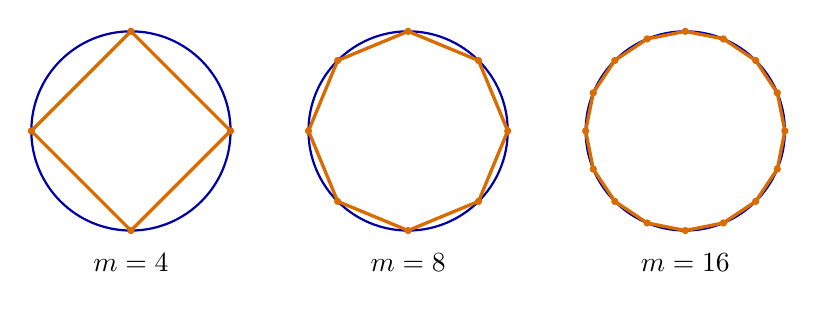
\begin{tikzpicture}[scale=1.1]
 \foreach \d/\m in {0/4,3.2/8,6.4/16}{
  \begin{scope}[xshift=\d cm]
   \draw[blue!65!black,thick] (0,0) circle (1.15);
   \pgfmathtruncatemacro{\last}{\m-1}
   \draw[orange!85!black,very thick]
     (0:1.15) \foreach \j in {1,...,\last}
       {-- ({360*\j/\m}:1.15)} -- cycle;
   \foreach \j in {0,...,\last}
     \fill[orange!85!black]
       ({360*\j/\m}:1.15) circle (1.2pt);
   \node[below] at (0,-1.3) {$m=\m$};
  \end{scope}
 }
\end{tikzpicture}
\caption{Łamane wpisane w okrąg jednostkowy
dla kolejnych podziałów diadycznych.
Długości wynoszą $4\sqrt2$,
$16\sin(\pi/8)$ i $32\sin(\pi/16)$,
a ich granicą jest $2\pi$.}
\label{ma2:fig:curve-circle-polygons}
\end{figure}

\paragraph{Prędkość i lokalny wkład.}
W punkcie różniczkowalności $\gamma$
mamy
\[
 \gamma(t+h)-\gamma(t)=h\gamma'(t)+o(|h|).
\]
Z nierówności odwrotnej do nierówności
trójkąta wynika
\[
 \|\gamma(t+h)-\gamma(t)\|_2
 =|h|\|\gamma'(t)\|_2+o(|h|).
\]
Sugeruje to, że długość można uzyskać
przez całkowanie modułu prędkości.
Dla krzywych klasy $C^1$ oraz absolutnie
ciągłych uzasadnimy to w twierdzeniach
\ref{ma2:thm:curve-c1-length}
i \ref{ma2:thm:curve-ac-length}.
Sama ciągłość i prostowalność nie wystarczą:
przykład \ref{ma2:ex:curve-cantor} pokazuje
drogę o dodatniej długości i prędkości
zerowej prawie wszędzie.
Nie można zatem w ogólności zastępować
definicji przez supremum wzorem całkowym.

\paragraph{Droga a jej geometryczny obraz.}
Niech $E=\gamma([a,b])$. Z rozdziału
\ref{ma2:ch:lebesgue-euclidean} wiemy,
że $\mathcal H^1$ mierzy geometryczny
obraz niezależnie od parametryzacji.
Nie uwzględnia liczby przejść przez
poszczególne części obrazu.
Długość drogi uwzględnia natomiast
powtórzenia. Możliwe jest więc, że
krzywa zamknięta ma niezerową długość
mimo zerowego przemieszczenia, a jej
długość jest większa od $\mathcal H^1(E)$.

\begin{przyklad}[Przejście tam i z powrotem]
\label{ma2:ex:curve-out-and-back}
Niech $\gamma:[0,2]\to\R^2$ będzie dana wzorem
\[
 \gamma(t)=
 \begin{cases}
 (t,0),&0\le t\le1,\\
 (2-t,0),&1\le t\le2.
 \end{cases}
\]
Obrazem jest odcinek jednostkowy $E$,
więc $\mathcal H^1(E)=1$ na mocy
\ref{ma2:prop:lebesgue-hausdorff-affine}.
Jednocześnie $L(\gamma)=2$:
podział $(0,1,2)$ daje sumę $2$,
a każda suma długości po dodaniu
punktu $1$ jest równa $2$, ponieważ
na obu częściach parametr jest monotoniczny.
Przemieszczenie $\gamma(2)-\gamma(0)$
jest zerowe. Dla $y\in E$ z wyjątkiem
punktu $(1,0)$ krotność wynosi $2$,
a w punkcie $(1,0)$ jest równa $1$.
Pojedynczy punkt nie wpływa na całkę
względem $\mathcal H^1$, toteż
\[
 L(\gamma)=2
 =\int_E N_\gamma(y)\,\mathrm d\mathcal H^1(y).
\]
Ogólną wersję tego wzoru wykażemy
w \ref{ma2:thm:curve-length-multiplicity}.
\end{przyklad}

\begin{figure}[htbp]
\centering
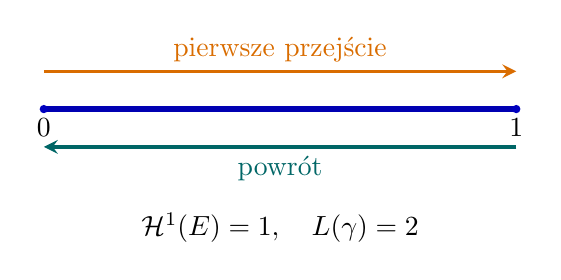
\begin{tikzpicture}[x=6cm,y=1cm,>=stealth]
 \draw[blue!70!black,line width=2pt] (0,0)--(1,0);
 \fill[blue!75!black] (0,0) circle (1.5pt);
 \fill[blue!75!black] (1,0) circle (1.5pt);
 \node[below] at (0,0) {$0$};
 \node[below] at (1,0) {$1$};
 \draw[orange!85!black,very thick,->] (0,.48)--(1,.48);
 \draw[teal!80!black,very thick,->] (1,-.48)--(0,-.48);
 \node[above,orange!85!black] at (.5,.48) {pierwsze przejście};
 \node[below,teal!80!black] at (.5,-.48) {powrót};
 \node[below] at (.5,-1.2)
 {$\mathcal H^1(E)=1,\quad L(\gamma)=2$};
\end{tikzpicture}
\caption{Dwa przejścia po jednym odcinku.
Strzałki przesunięto dla czytelności:
obie oznaczają ruch po tym samym zbiorze.}
\label{ma2:fig:curve-out-and-back}
\end{figure}

Dla całki krzywoliniowej pierwszego
rodzaju będziemy ważyć długość drogi
wartością gęstości. Dla całki drugiego
rodzaju istotna będzie także orientacja:
przejście odcinka w przeciwnym kierunku
odwraca znak wkładu pola wektorowego.
Rozróżnienie to rozwiniemy w rozdziale
\ref{ma2:ch:line-integrals}.

\section{Długość jako wahanie}

\begin{definicja}
\label{ma2:def:curve-variation}
Niech $a<b$ i $\gamma:[a,b]\to\R^n$ będzie ciągła.
Dla podziału $P=(t_0,\ldots,t_m)$, gdzie
$a=t_0<\cdots<t_m=b$, określamy
\[
 L_P(\gamma)=\sum_{j=1}^m
 \|\gamma(t_j)-\gamma(t_{j-1})\|_2,\qquad
 L(\gamma)=\sup_P L_P(\gamma).
\]
Krzywą nazywamy prostowalną, jeżeli $L(\gamma)<\infty$.
Długość ograniczenia do $[u,v]$ oznaczamy
$L_{[u,v]}(\gamma)$, przyjmując $L_{[u,u]}(\gamma)=0$.
Jest to definicja z
\atlasref{AM1-33::ma1:def:curve-length}{AM I, rozdział 33},
czyli wahanie całkowite odwzorowania $\gamma$.
\end{definicja}

\begin{stwierdzenie}
\label{ma2:prop:curve-length-basic}
Dla $a\le u\le v\le w\le b$ zachodzi
\[
 \|\gamma(v)-\gamma(u)\|_2\le L_{[u,v]}(\gamma),
 \qquad
 L_{[u,w]}(\gamma)=L_{[u,v]}(\gamma)+L_{[v,w]}(\gamma).
\]
Krzywa jest prostowalna wtedy i tylko wtedy,
gdy każda jej współrzędna ma ograniczone wahanie.
\end{stwierdzenie}
\begin{proof}
Pierwsza nierówność wynika z podziału złożonego
tylko z końców. Dodanie punktu do podziału nie
zmniejsza sumy długości dzięki nierówności
trójkąta. Wstawiając $v$ do podziału $[u,w]$,
otrzymujemy oszacowanie z góry przez sumę
długości obu części. W przeciwnym kierunku
łączymy dowolne podziały obu części i przechodzimy
do supremum, również gdy jedno z nich jest nieskończone.

Dla $\gamma=(\gamma_1,\ldots,\gamma_n)$ z nierówności
$|z_i|\le\|z\|_2\le\sum_i|z_i|$ wynika
\[
 \max_i\operatorname{Var}_{[a,b]}\gamma_i
 \le L(\gamma)\le
 \sum_{i=1}^n\operatorname{Var}_{[a,b]}\gamma_i,
\]
gdzie $\operatorname{Var}$ oznacza wahanie całkowite.
\end{proof}

\begin{twierdzenie}[Niezmienniczość przy reparametryzacji]
\label{ma2:thm:curve-reparam}
Niech $c<d$. Jeżeli $\varphi:[c,d]\to[a,b]$ jest ciągła,
monotoniczna (niemalejąca lub nierosnąca)
i surjektywna, to $L(\gamma\circ\varphi)=L(\gamma)$.
Nie zakładamy różniczkowalności ani ścisłej monotoniczności.
\end{twierdzenie}
\begin{proof}
Obraz dowolnego podziału $[c,d]$ przez $\varphi$,
po usunięciu powtórzeń i ewentualnym odwróceniu
kolejności, jest podziałem $[a,b]$. Sumy długości
są równe, więc $L(\gamma\circ\varphi)\le L(\gamma)$.
Odwrotnie, dla każdego podziału $[a,b]$ wybieramy
przeciwobrazy kolejnych punktów w odpowiedniej
kolejności, z końcami $c,d$. Surjektywność gwarantuje
ich istnienie, monotoniczność uporządkowanie.
Przejście do supremum daje drugą nierówność.
\end{proof}

\begin{stwierdzenie}[Przybliżanie długości łamanymi]
\label{ma2:prop:curve-polygon-limit}
Niech $(P_j)$ będzie ciągiem podziałów $[a,b]$
i niech $t_{j,i}$ oznaczają kolejne punkty $P_j$.
Jeżeli średnice podziałów
$\|P_j\|=\max_i(t_{j,i}-t_{j,i-1})$ dążą do zera, to
$L_{P_j}(\gamma)\to L(\gamma)$, również wtedy,
gdy długość jest nieskończona.
\end{stwierdzenie}
\begin{proof}
Ustalmy dowolny podział $Q$ o $k$ punktach wewnętrznych.
Niech $\omega(\delta)=\sup\{\|\gamma(u)-\gamma(v)\|_2:
u,v\in[a,b],\ |u-v|\le\delta\}$.
Z jednostajnej ciągłości $\gamma$ mamy
$\omega(\delta)\to0$ przy $\delta\downarrow0$.
Wstawienie jednego punktu do przedziału podziału
$P_j$ (lub jego rozdrobnienia) zwiększa sumę
długości o co najwyżej $2\omega(\|P_j\|)$,
gdyż dodane odcinki mają długość nie większą
od $\omega(\|P_j\|)$.
Stąd
\[
 L_Q(\gamma)\le L_{P_j\cup Q}(\gamma)
 \le L_{P_j}(\gamma)+2k\omega(\|P_j\|).
\]
Przechodząc do granicy dolnej, otrzymujemy
$L_Q(\gamma)\le\liminf_j L_{P_j}(\gamma)$.
Bierzemy supremum po $Q$, a przeciwną nierówność
otrzymujemy wprost z definicji długości.
\end{proof}

\begin{figure}[htbp]
\centering
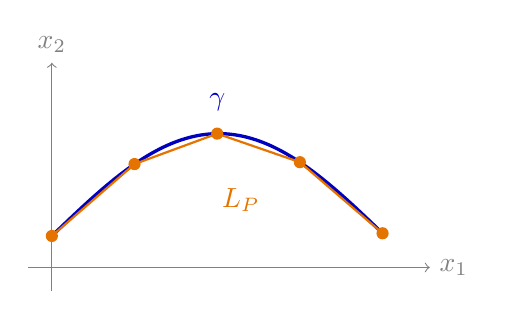
\begin{tikzpicture}[scale=2]
 \draw[->,gray] (-.15,0)--(2.4,0) node[right] {$x_1$};
 \draw[->,gray] (0,-.15)--(0,1.3) node[above] {$x_2$};
 \draw[blue!75!black,very thick,domain=0:2.1,samples=90]
  plot (\x,{.2+.65*sin(85*\x)});
 \draw[orange!90!black,thick] (0,.2)
 -- (.525,{.2+.65*sin(85*.525)})
 -- (1.05,{.2+.65*sin(85*1.05)})
 -- (1.575,{.2+.65*sin(85*1.575)})
 -- (2.1,{.2+.65*sin(85*2.1)});
 \foreach \t in {0,.525,1.05,1.575,2.1}
  \fill[orange!90!black] (\t,{.2+.65*sin(85*\t)}) circle (1.1pt);
 \node[blue!75!black] at (1.05,1.05) {$\gamma$};
 \node[orange!90!black] at (1.2,.43) {$L_P$};
\end{tikzpicture}
\caption{Łamana wpisana w krzywą. Zmniejszanie
średnicy podziału prowadzi do długości krzywej,
zgodnie z \ref{ma2:prop:curve-polygon-limit}.}
\label{ma2:fig:curve-polygon}
\end{figure}

\section{Krzywe klasy \texorpdfstring{$C^1$}{C1} i absolutnie ciągłe}

\begin{twierdzenie}
\label{ma2:thm:curve-c1-length}
Jeżeli $\gamma:[a,b]\to\R^n$ jest klasy $C^1$
(z pochodnymi jednostronnymi na końcach), to
\[
 L(\gamma)=\int_a^b\|\gamma'(t)\|_2\,\mathrm d\lambda_1(t)
 =\int_a^b\sqrt{\sum_{i=1}^n|\gamma_i'(t)|^2}\,
 \mathrm d\lambda_1(t).
\]
Nie trzeba zakładać, że $\gamma'(t)\ne0$.
\end{twierdzenie}
Dowód podano w
\atlasref{AM1-33::ma1:thm:curve-length}{AM I, rozdział 33}.
Ciągłość funkcji podcałkowej zapewnia zgodność
całek Riemanna i Lebesgue'a na mocy
\ref{ma2:thm:lebesgue-jordan-agreement}.
Addytywność długości rozszerza wzór na krzywe
ciągłe, których ograniczenia do domkniętych
podprzedziałów pewnego skończonego podziału
są klasy $C^1$ (z pochodnymi jednostronnymi
na końcach tych podprzedziałów).

\begin{definicja}
\label{ma2:def:curve-ac}
Krzywa $\gamma:[a,b]\to\R^n$ jest absolutnie
ciągła, jeżeli dla każdego
$\varepsilon>0$ istnieje $\delta>0$ takie, że
dla każdej skończonej rodziny przedziałów
$[u_j,v_j]\subseteq[a,b]$ o parami rozłącznych
wnętrzach z $\sum_j(v_j-u_j)<\delta$ zachodzi
\[
 \sum_j\|\gamma(v_j)-\gamma(u_j)\|_2<\varepsilon.
\]
Równoważnie każda współrzędna jest absolutnie
ciągła; wynika to z nierówności normowych użytych
w \ref{ma2:prop:curve-length-basic}, wybierając
wspólne $\delta$ dla skończenie wielu współrzędnych
przy tolerancji $\varepsilon/n$ dla każdej z nich.
Warunek dla pojedynczego przedziału implikuje
jednostajną ciągłość $\gamma$.
\end{definicja}

\begin{twierdzenie}[Długość krzywej absolutnie ciągłej]
\label{ma2:thm:curve-ac-length}
Jeżeli $\gamma$ jest absolutnie ciągła, to jej
pochodna istnieje prawie wszędzie, $\|\gamma'\|_2$
jest całkowalna i
\[
 L_{[u,v]}(\gamma)=
 \int_{[u,v]}\|\gamma'(t)\|_2\,\mathrm d\lambda_1(t)
 \qquad(a\le u\le v\le b).
\]
W szczególności $\gamma$ jest prostowalna.
\end{twierdzenie}
\begin{proof}
Twierdzenie o funkcji pierwotnej
\atlasref{AM1-37::ma1:kh:thm:ac-lebesgue-primitive}{AM I, rozdział 37}
stosujemy do każdej współrzędnej. Poza sumą
skończenie wielu zbiorów zerowych istnieją
wszystkie pochodne. Przyjmujemy $\gamma'=0$ na
pozostałym zbiorze zerowym (w tym na końcach).
Mierzalność i całkowalność współrzędnych pochodnej
wynikają z przywołanego twierdzenia, więc
$\|\gamma'\|_2\le\sum_i|\gamma_i'|$ jest całkowalna.
Dla $u<v$ i dowolnego jednostkowego $e\in\R^n$
mamy z liniowości całki
\[
 \langle e,\gamma(v)-\gamma(u)\rangle
 =\int_{[u,v]}\langle e,\gamma'(t)\rangle\,\mathrm d\lambda_1(t)
 \le\int_{[u,v]}\|\gamma'(t)\|_2\,\mathrm d\lambda_1(t).
\]
Biorąc supremum po $e$, a następnie sumując
nierówności dla podziału, dostajemy
$L(\gamma)\le\int_{[a,b]}\|\gamma'\|_2\,\mathrm d\lambda_1$.

Dla nierówności odwrotnej dzielimy $[a,b]$ na
$2^j$ równych przedziałów. Niech $q_j(t)$ na
każdym półotwartym przedziale $[u,v)$ podziału
będzie równe $(\gamma(v)-\gamma(u))/(v-u)$.
W punkcie $b$ przyjmujemy $q_j(b)=0$.
W punkcie różniczkowalności $t\in(a,b)$ mamy
$q_j(t)\to\gamma'(t)$: dla końców przedziału
zawierającego $t$ rozwijamy
$\gamma(z)=\gamma(t)+\gamma'(t)(z-t)+o(|z-t|)$.
Suma modułów reszt podzielona przez $v-u$ dąży
do zera, ponieważ $|v-t|+|u-t|=v-u$.
Funkcje $\|q_j\|_2$ są mierzalne, nieujemne,
a każda ich całka jest sumą długości odcinków
odpowiedniej łamanej wpisanej.
Lemat Fatou \ref{ma2:thm:lebesgue-fatou} daje
\[
 \int_{[a,b]}\|\gamma'(t)\|_2\,\mathrm d\lambda_1(t)
 \le\liminf_j\int_{[a,b]}\|q_j(t)\|_2\,\mathrm d\lambda_1(t)
 \le L(\gamma).
\]
Tak samo postępujemy na każdym niezdegenerowanym
podprzedziale, ponieważ ograniczenie pozostaje
absolutnie ciągłe. Dla $u=v$ obie strony są zerowe.
\end{proof}

\section{Parametryzacja długością łuku}

Parametr $s(t)$ oznacza długość przebytą
od początku drogi do chwili $t$, a nie
odległość od punktu początkowego.
Na odcinku czasu, w którym punkt
pozostaje nieruchomy, parametr $s$
jest stały. Parametryzacja długością
łuku usuwa takie postoje i zastępuje
zmienne tempo ruchem o jednostkowej
prędkości prawie wszędzie. Nie usuwa
natomiast przejść powrotnych ani
samoprzecięć krzywej.

\begin{twierdzenie}
\label{ma2:thm:curve-arclength}
Niech $\gamma:[a,b]\to\R^n$ będzie ciągła
i prostowalna, a $\ell=L(\gamma)$.
Funkcja $s(t)=L_{[a,t]}(\gamma)$ jest ciągła,
niemalejąca i odwzorowuje $[a,b]$ na $[0,\ell]$.
Istnieje dokładnie jedna funkcja
$\widehat\gamma:[0,\ell]\to\R^n$ taka, że
$\gamma(t)=\widehat\gamma(s(t))$.
Jest ona $1$-Lipschitzowska i dla
$0\le p\le q\le\ell$ spełnia
$L_{[p,q]}(\widehat\gamma)=q-p$.
Gdy $\ell>0$, zachodzi także
$\|\widehat\gamma'(s)\|_2=1$ prawie wszędzie.
\end{twierdzenie}
\begin{proof}
Monotoniczność i równość
$s(v)-s(u)=L_{[u,v]}(\gamma)$ wynikają z
\ref{ma2:prop:curve-length-basic}.
Dla dowolnego $\varepsilon>0$ i $a<t\le b$
wybieramy podział $[a,t]$ o sumie
większej od $s(t)-\varepsilon$. Gdy $u<t$ jest
bliskie $t$ i leży za przedostatnim punktem,
zastąpienie ostatniego punktu przez $u$ daje
podział $[a,u]$ o sumie dążącej do pierwotnej,
z ciągłości $\gamma$. Stąd
$\lim_{u\uparrow t}s(u)=s(t)$.
Dla krzywej $\widetilde\gamma(r)=\gamma(a+b-r)$
funkcja długości wynosi
$\widetilde s(r)=L_{[a,r]}(\widetilde\gamma)
=\ell-s(a+b-r)$, na mocy addytywności długości
i \ref{ma2:thm:curve-reparam}. Jej lewostronna
ciągłość dla $a<r\le b$ daje prawostronną
ciągłość $s$ dla $a\le t<b$.
Surjektywność wynika z twierdzenia o wartości pośredniej.

Jeżeli $s(u)=s(v)$ przy $u\le v$, to długość
$[u,v]$ jest zero, więc $\gamma(u)=\gamma(v)$.
Możemy zatem jednoznacznie określić
$\widehat\gamma(s(t))=\gamma(t)$.
Dla $p<q$ wybieramy $u<v$ z $s(u)=p$, $s(v)=q$.
Wówczas
\[
 \|\widehat\gamma(q)-\widehat\gamma(p)\|_2
 \le L_{[u,v]}(\gamma)=q-p.
\]
Ponieważ $s|_{[u,v]}$ jest ciągłą monotoniczną
surjekcją na $[p,q]$, twierdzenie
\ref{ma2:thm:curve-reparam} daje
$L_{[p,q]}(\widehat\gamma)=q-p$.
Jeżeli $\ell>0$, warunek Lipschitza zapewnia
absolutną ciągłość wprost z definicji
\ref{ma2:def:curve-ac}. Mamy
$\|\widehat\gamma'\|_2\le1$ prawie wszędzie,
a z \ref{ma2:thm:curve-ac-length} jej całka
na $[0,\ell]$ wynosi $\ell$.
Całka funkcji nieujemnej $1-\|\widehat\gamma'\|_2$
jest zero, co daje tezę.
Dla $\ell=0$ krzywa jest stała i faktoryzacja
dotyczy jednopunktowego przedziału.
\end{proof}

\begin{wniosek}
\label{ma2:cor:curve-regular-arclength}
Krzywą klasy $C^1$ nazywamy regularną, jeżeli jej
pochodna nie znika w żadnym punkcie przedziału.
Jeżeli $\gamma$ jest klasy $C^1$ i $\gamma'(t)\ne0$
na całym przedziale, to $\widehat\gamma$ jest klasy
$C^1$ i ma prędkość jednostkową w każdym punkcie
(z pochodnymi jednostronnymi na końcach).
\end{wniosek}
\begin{proof}
Z \ref{ma2:thm:curve-c1-length} i podstawowego
twierdzenia rachunku całkowego
$s'(t)=\|\gamma'(t)\|_2>0$. Funkcja $s$ jest
ściśle rosnąca i ma odwrotność klasy $C^1$
we wnętrzu; wzór na pochodną odwrotności
przedłuża się jednostronnie na końce,
gdyż $s'$ jest tam ciągła i dodatnia.
Reguła łańcuchowa dla $\widehat\gamma=\gamma\circ s^{-1}$
daje $\widehat\gamma'(s(t))=\gamma'(t)/\|\gamma'(t)\|_2$.
\end{proof}

\begin{wniosek}[Regularność parametru długości]
\label{ma2:cor:curve-ac-arclength}
Niech $\gamma$ będzie ciągła i prostowalna.
Funkcja $s(t)=L_{[a,t]}(\gamma)$ jest absolutnie
ciągła wtedy i tylko wtedy, gdy $\gamma$ jest
absolutnie ciągła.
\end{wniosek}
\begin{proof}
Jeżeli $\gamma$ jest absolutnie ciągła, to
\ref{ma2:thm:curve-ac-length} daje
$s(t)=\int_{[a,t]}\|\gamma'(u)\|_2\,\mathrm d\lambda_1(u)$.
Całka funkcji całkowalnej jest absolutnie ciągła
na mocy
\atlasref{AM1-37::ma1:kh:thm:ac-lebesgue-primitive}{twierdzenia o funkcji pierwotnej}.
Odwrotnie, dla $u\le v$ mamy
$\|\gamma(v)-\gamma(u)\|_2\le s(v)-s(u)$
z \ref{ma2:prop:curve-length-basic}.
Sumując te nierówności i stosując definicję
absolutnej ciągłości do $s$, otrzymujemy
absolutną ciągłość $\gamma$.
\end{proof}

\begin{przyklad}[Ten sam łuk przebyty w różnym tempie]
\label{ma2:ex:curve-arclength-variable-speed}
Niech $H:[0,1]\to\R^3$,
$H(q)=(\cos(2\pi q),\sin(2\pi q),2q)$.
Rozważmy $\gamma_1(t)=H(t)$ oraz
$\gamma_2(t)=H(t^2)$ dla $0\le t\le1$.
Krzywe mają ten sam obraz i tę samą
kolejność przejścia, ponieważ
$t\mapsto t^2$ jest rosnącą surjekcją
na $[0,1]$. Z twierdzenia
\ref{ma2:thm:curve-reparam} ich długości
są więc równe.
Rachunek pochodnych daje
\[
 \|H'(q)\|_2=\ell=\sqrt{4\pi^2+4},
 \qquad
 \|\gamma_1'(t)\|_2=\ell,\quad
 \|\gamma_2'(t)\|_2=2t\ell.
\]
Na mocy \ref{ma2:thm:curve-c1-length}
funkcje długości to odpowiednio
$s_1(t)=\ell t$ oraz $s_2(t)=\ell t^2$.
Obie parametryzacje prowadzą do tej
samej funkcji
\[
 \widehat\gamma(s)=H(s/\ell),\qquad 0\le s\le\ell.
\]
Jest ona klasy $C^1$ i ma jednostkową
prędkość, chociaż $\gamma_2'(0)=0$.
Regularność pierwotnej krzywej jest
więc warunkiem wystarczającym, lecz
nie koniecznym dla gładkości parametryzacji
długością łuku (por.
\ref{ma2:cor:curve-regular-arclength} oraz
\ref{ma2:ex:curve-cusp}).
\end{przyklad}

\begin{figure}[htbp]
\centering
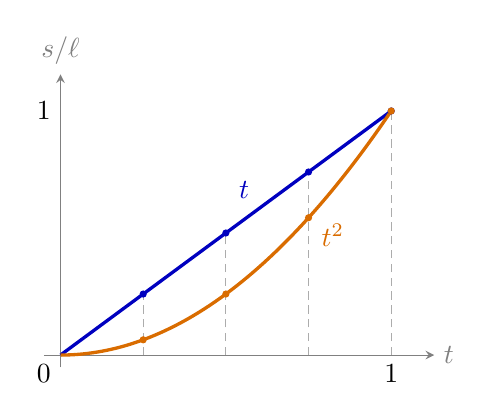
\begin{tikzpicture}[x=4.2cm,y=3.1cm,>=stealth]
 \draw[->,gray] (-.05,0)--(1.13,0) node[right] {$t$};
 \draw[->,gray] (0,-.05)--(0,1.15) node[above] {$s/\ell$};
 \draw[blue!75!black,very thick] (0,0)--(1,1);
 \draw[orange!85!black,very thick,domain=0:1,samples=61]
  plot (\x,{\x*\x});
 \foreach \t in {.25,.5,.75,1}{
  \draw[gray!65,densely dashed] (\t,0)--(\t,\t);
  \fill[blue!75!black] (\t,\t) circle (1.3pt);
  \fill[orange!85!black] (\t,{\t*\t}) circle (1.3pt);
 }
 \node[blue!75!black,above left] at (.6,.6) {$t$};
 \node[orange!85!black,below right] at (.76,.5776) {$t^2$};
 \node[below left] at (0,0) {$0$};
 \node[below] at (1,0) {$1$};
 \node[left] at (0,1) {$1$};
\end{tikzpicture}
\caption{Znormalizowane funkcje długości
z przykładu \ref{ma2:ex:curve-arclength-variable-speed}.
W chwili $t=1/2$ pierwszy ruch przebył
połowę, a drugi jedną czwartą długości łuku.}
\label{ma2:fig:curve-arclength-variable-speed}
\end{figure}

\section{Długość drogi i miara Hausdorffa obrazu}

Stosujemy normalizację $\mathcal H^1$ z
\atlasref{ME-26::thm:hausdorff-line-26}{teorii miary i całki},
dla której $\mathcal H^1$ na prostej zgadza się
z miarą Lebesgue'a na zbiorach mierzalnych.
Niech teraz $\gamma$ będzie prostowalna i $\ell=L(\gamma)$.
Dla $\ell>0$ parametryzacja długością łuku jest
$1$-Lipschitzowska, więc
\atlasref{ME-26::thm:hausdorff-lipschitz-26}{nierówność Lipschitza dla miary Hausdorffa}
daje
\[
 \mathcal H^1(\gamma([a,b]))\le
 \mathcal H^1([0,\ell])=\ell.
\]
Dla krzywej stałej nierówność też zachodzi,
gdyż punkt ma zerową miarę $\mathcal H^1$.

\begin{stwierdzenie}[Elementarny wzór dla krzywej prostej]
\label{ma2:prop:simple-curve-hausdorff}
Jeżeli $\gamma:[a,b]\to\R^n$ jest ciągła
i różnowartościowa, to
\[
 L(\gamma)=\mathcal H^1(\gamma([a,b])),
\]
również gdy obie strony są nieskończone.
\end{stwierdzenie}
\begin{proof}
Nierówność $\mathcal H^1(\gamma([a,b]))\le L(\gamma)$
wykazaliśmy powyżej dla krzywych prostowalnych,
a dla nieskończonej długości jest automatyczna.

Ustalmy podział $P=(t_0,\ldots,t_m)$ i oznaczmy
$E_i=\gamma([t_{i-1},t_i])$.
Każdy $E_i$ jest zwarty i spójny. Jeśli
$z_i=\gamma(t_i)-\gamma(t_{i-1})$, to $z_i\ne0$
z różnowartościowości krzywej.
Rzut skalarny $x\mapsto\langle x,z_i/\|z_i\|_2\rangle$
jest $1$-Lipschitzowski. Jego obraz $E_i$ jest
spójnym zbiorem na prostej zawierającym obrazy obu
końców, a zatem zawiera przedział długości
$\|z_i\|_2$. Nierówność Lipschitza dla $\mathcal H^1$
i zgodność $\mathcal H^1$ z miarą Lebesgue'a na
prostej dają $\mathcal H^1(E_i)\ge\|z_i\|_2$.
Z różnowartościowości wynika, że różne $E_i$
mogą przecinać się jedynie w obrazach końców
podprzedziałów. Są to zbiory zerowej miary
$\mathcal H^1$. Skończona addytywność miary
na zbiorach borelowskich
(\atlasref{ME-26::thm:hausdorff-borel-26}{ME 26})
daje więc
\[
 \mathcal H^1(\gamma([a,b]))
 =\sum_{i=1}^m\mathcal H^1(E_i)
 \ge L_P(\gamma).
\]
Przechodzimy do supremum po wszystkich podziałach.
Dowód nie korzysta ze wzoru na pole z krotnością.
\end{proof}

\begin{twierdzenie}[Długość z krotnością]
\label{ma2:thm:curve-length-multiplicity}
Niech $\gamma$ będzie ciągła i prostowalna.
Dla $y\in\R^n$ niech
$N_\gamma(y)=\#\{t\in[a,b]:\gamma(t)=y\}$,
z wartością $+\infty$ dla nieskończonego włókna.
Wówczas $N_\gamma$ jest funkcją borelowską i
\[
 L(\gamma)=\int_{\R^n}N_\gamma(y)\,\mathrm d\mathcal H^1(y).
\]
Jeżeli $\gamma$ jest różnowartościowa, to
$L(\gamma)=\mathcal H^1(\gamma([a,b]))$.
\end{twierdzenie}
\begin{proof}
Najpierw wykażemy borelowskość krotności. Dla
liczb naturalnych $k,j\ge1$ niech $E_{k,j}$
będzie zbiorem wszystkich $(t_1,\ldots,t_k)\in[a,b]^k$
spełniających $|t_p-t_q|\ge1/j$ dla $p\ne q$
oraz $\gamma(t_1)=\cdots=\gamma(t_k)$.
Jest to zbiór zwarty, bo warunki określają
zbiory domknięte. Jego obraz $B_{k,j}$ przez
ciągłe odwzorowanie $(t_1,\ldots,t_k)\mapsto\gamma(t_1)$
jest zwarty. Zachodzi
\[
 \{y:N_\gamma(y)\ge k\}=\bigcup_{j\ge1}B_{k,j},
\]
ponieważ dowolne $k$ różnych punktów włókna
ma dodatnią minimalną odległość (dla $k=1$
warunek odległości jest pusty). Wszystkie zbiory
$\{N_\gamma\ge k\}$ są borelowskie, co dowodzi
mierzalności funkcji o wartościach w
$\mathbb N_0\cup\{+\infty\}$.
Ten argument nie wymaga prostowalności.

Oznaczmy $\ell=L(\gamma)$.
Dla $\ell=0$ krotność jest zero poza jednym
punktem, więc całka jest zero.
Niech $\ell>0$. Parametryzację $\widehat\gamma$
z \ref{ma2:thm:curve-arclength} przedłużamy na
$\R$ wartościami stałymi poza $[0,\ell]$;
przedłużenie jest $1$-Lipschitzowskie jako
złożenie z rzutem na przedział.
Stosujemy wzór na pole z krotnością
\atlasref{ME-28::thm:lipschitz-area-coarea-28}{ME 28}
dla $k=1$, zbioru $E=[0,\ell]$ i funkcji równej $1$.
Z definicji jakobianu
(\atlasref{ME-28::def:k-jacobian-28}{ME 28})
dla macierzy kolumnowej $\widehat\gamma'(s)$
otrzymujemy jakobian jednowymiarowy
$\sqrt{\widehat\gamma'(s)^{\mathsf T}\widehat\gamma'(s)}
=\|\widehat\gamma'(s)\|_2$ prawie wszędzie.
Dostajemy
$\int_{\R^n}N_{\widehat\gamma}\,\mathrm d\mathcal H^1=\ell$.

Włókna niemalejącej funkcji $s$ są przedziałami.
Tych zawierających więcej niż jeden punkt
jest co najwyżej przeliczalnie wiele, gdyż
mają parami rozłączne niepuste wnętrza,
z których każde zawiera liczbę wymierną.
Poza obrazami tych przeliczalnie wielu wartości
przez $\widehat\gamma$ krotności
$N_\gamma$ i $N_{\widehat\gamma}$ są równe.
Ten zbiór wyjątkowy ma zerową miarę $\mathcal H^1$
na mocy
\atlasref{ME-26::cor:hausdorff-singletons-auditVI}{ME 26}.
Ponieważ obie funkcje krotności są borelowskie
(na mocy pierwszej części dowodu) i równe prawie
wszędzie, ich całki są równe.
Dla krzywej różnowartościowej $N_\gamma$ jest
funkcją charakterystyczną jej zwartego obrazu.
\end{proof}

\begin{wniosek}[Kiedy długość jest miarą obrazu?]
\label{ma2:cor:curve-length-image-equality}
Dla ciągłej krzywej prostowalnej o obrazie $E$
równość $L(\gamma)=\mathcal H^1(E)$ zachodzi
wtedy i tylko wtedy, gdy $N_\gamma(y)=1$
dla $\mathcal H^1$-prawie każdego $y\in E$.
\end{wniosek}
\begin{proof}
Na $E$ mamy $N_\gamma\ge1$, poza $E$ mamy zero.
Z twierdzenia \ref{ma2:thm:curve-length-multiplicity}
i skończoności długości wynika
\[
 L(\gamma)-\mathcal H^1(E)=
 \int_E (N_\gamma(y)-1)\,\mathrm d\mathcal H^1(y).
\]
Całka funkcji nieujemnej jest zerowa wtedy i tylko
wtedy, gdy funkcja jest zerowa prawie wszędzie.
\end{proof}

\section{Przykłady}

\begin{przyklad}[Ten sam okrąg, różne długości dróg]
\label{ma2:ex:curve-circle-multiplicity}
Dla $R>0$ i liczby naturalnej $m\ge1$ krzywa
$\gamma_m(t)=R(\cos t,\sin t)$ na $[0,2m\pi]$
ma prędkość $R$, więc jej długość wynosi $2m\pi R$
na mocy \ref{ma2:thm:curve-c1-length}.
Jej obraz jest zawsze tym samym okręgiem.
Na okręgu krotność jest równa $m$ poza punktem
$(R,0)$, w którym wynosi $m+1$. Poza okręgiem
jest równa zero. Punkt ma zerową miarę
$\mathcal H^1$, więc \ref{ma2:thm:curve-length-multiplicity}
dla $m=1$ daje miarę okręgu $2\pi R$, a dla dowolnego
$m$ odzyskujemy długość $2m\pi R$.
\end{przyklad}

\begin{przyklad}[Helisa]
\label{ma2:ex:curve-helix}
Dla $R>0$, $h\in\R$ i $T>0$ krzywa
$\gamma(t)=(R\cos t,R\sin t,ht)$, $0\le t\le T$,
ma pochodną $(-R\sin t,R\cos t,h)$.
Jej długość wynosi $T\sqrt{R^2+h^2}$,
a parametr długości to $s=t\sqrt{R^2+h^2}$,
na mocy \ref{ma2:thm:curve-c1-length}.
\end{przyklad}

\begin{figure}[htbp]
\centering
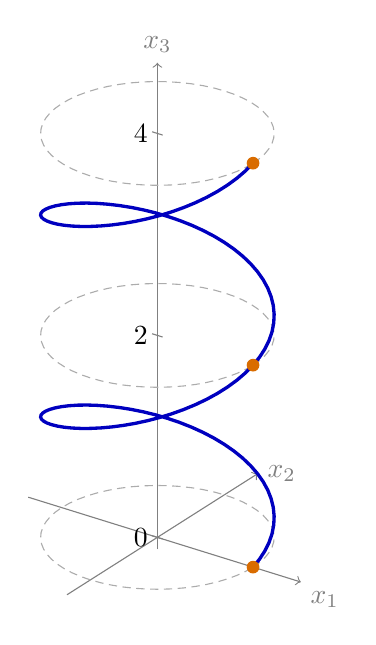
\begin{tikzpicture}[x={(0.90cm,-0.28cm)},y={(0.63cm,0.40cm)},
 z={(0cm,0.95cm)},scale=1.35]
 \draw[->,gray] (-1.35,0,0)--(1.5,0,0) node[below right] {$x_1$};
 \draw[->,gray] (0,-1.35,0)--(0,1.5,0) node[right] {$x_2$};
 \draw[->,gray] (0,0,-.12)--(0,0,4.7) node[above] {$x_3$};
 \foreach \h in {0,2,4}{
  \draw[gray!65,densely dashed,domain=0:360,samples=61]
   plot ({cos(\x)},{sin(\x)},\h);
  \draw[gray] (-.055,0,\h)--(.055,0,\h);
  \node[left] at (0,0,\h) {$\h$};
 }
 \draw[blue!75!black,very thick,domain=0:720,samples=121,variable=\t]
  plot ({cos(\t)},{sin(\t)},{\t/180});
 \foreach \h in {0,2,4}
  \fill[orange!85!black] (1,0,\h) circle[radius=1.7pt];
\end{tikzpicture}
\caption{Helisa o promieniu $1$ i skoku $2$,
z parametrem $t\in[0,4\pi]$ i $h=1/\pi$
(przykład \ref{ma2:ex:curve-helix}).
Punkty wyróżnione odpowiadają pełnym obrotom.
Przerywane okręgi pomocnicze leżą na wysokościach $0,2,4$.}
\label{ma2:fig:curve-helix}
\end{figure}

\begin{przyklad}[Krzywa prostowalna o pochodnej zerowej prawie wszędzie]
\label{ma2:ex:curve-cantor}
Niech $\kappa$ będzie bezatomową miarą Cantora,
skupioną na klasycznym zbiorze Cantora $K$,
z \atlasref{ME-17::ex:cantor-measure-17}{ME 17}.
Dystrybuanta $C(t)=\kappa([0,t])$, $0\le t\le1$,
jest ciągła i niemalejąca, $C(0)=0$, $C(1)=1$.
Ciągłość wynika z braku atomów, a poza $K$ funkcja
jest lokalnie stała. Ponieważ $\lambda_1(K)=0$ (por. konstrukcję miary
Cantora w ME 17), mamy $C'=0$ prawie wszędzie.
Dla krzywej $\gamma(t)=(C(t),0)\in\R^2$
każda suma długości w podziale jest równa
$\sum_j(C(t_j)-C(t_{j-1}))=1$.
W konsekwencji
\[
 L(\gamma)=1,\qquad
 \int_{[0,1]}\|\gamma'(t)\|_2\,\mathrm d\lambda_1(t)=0.
\]
Krzywa nie jest absolutnie ciągła, gdyż
przeczyłoby to \ref{ma2:thm:curve-ac-length}.
Jej parametr długości to $s(t)=C(t)$,
a $\widehat\gamma(s)=(s,0)$.
Ten przykład pokazuje, że prostowalność
nie zapewnia wzoru na długość przez całkę
z prędkości w pierwotnym parametrze.
\end{przyklad}

\begin{przyklad}[Punkt nieregularny i parametr długości]
\label{ma2:ex:curve-cusp}
Niech $\gamma(t)=(t^2,t^3)$ dla $-1\le t\le1$.
Mimo że $\gamma'(0)=0$, krzywa jest prostowalna
jako krzywa klasy $C^1$. Jej prędkość wynosi
$|t|\sqrt{4+9t^2}$, a długość
\[
 L(\gamma)=2\int_0^1 t\sqrt{4+9t^2}\,\mathrm d\lambda_1(t)
 =\frac{2}{27}(13^{3/2}-8).
\]
Ostatnią równość otrzymujemy przez podstawienie
$u=4+9t^2$. Parametr długości $s$ jest ściśle
rosnący (prędkość jest dodatnia poza pojedynczym
punktem). W punkcie $s_0=s(0)$ parametryzacja
$\widehat\gamma$ nie jest różniczkowalna.
Istotnie, dla $t\ne0$
\[
 \frac{\widehat\gamma(s(t))-\widehat\gamma(s_0)}
 {s(t)-s_0}
 =\frac{(t^2,t^3)}
 {\operatorname{sgn}(t)\int_0^{|t|}u\sqrt{4+9u^2}\,
 \mathrm d\lambda_1(u)}.
\]
Ponieważ dla $0\le u\le|t|$ mamy
$2\le\sqrt{4+9u^2}\le\sqrt{4+9t^2}$,
całka podzielona przez $t^2$ dąży do $1$.
Ilorazy różnicowe mają granice jednostronne
$(-1,0)$ i $(1,0)$, zatem pochodna nie istnieje.
Warunek regularności w
\ref{ma2:cor:curve-regular-arclength}
nie jest więc zbędny.
\end{przyklad}

\begin{przyklad}[Ciągły wykres nieprostowalny]
\label{ma2:ex:curve-infinite-oscillations}
Połóżmy $g(0)=0$ i $g(t)=t\sin(1/t)$ dla $0<t\le1$.
Krzywa $\gamma(t)=(t,g(t))$ jest ciągła,
ponieważ $|g(t)|\le t$. Dla
$t_j=(\pi/2+j\pi)^{-1}$, $j\ge0$, mamy
$g(t_j)=(-1)^j t_j$.
Punkty $t_j$ maleją do zera, a długość łamanej
przez $\gamma(t_N),\ldots,\gamma(t_0)$ jest co najmniej
\[
 \sum_{j=0}^{N-1}|g(t_{j+1})-g(t_j)|
 =\sum_{j=0}^{N-1}(t_j+t_{j+1}).
\]
Szereg jest rozbieżny przez porównanie z szeregiem
harmonicznym. Po uzupełnieniu punktów o końce
$0,1$ dostajemy podziały o dowolnie dużych sumach.
Krzywa nie jest prostowalna. Ponieważ pierwsza
współrzędna jest ściśle rosnąca, krzywa jest
różnowartościowa, a z
\ref{ma2:prop:simple-curve-hausdorff} wynika także
$\mathcal H^1(\gamma([0,1]))=+\infty$.
\end{przyklad}

W kolejnym rozdziale rozwiniemy całkowanie
wielokrotne. Długość i miara $\mathcal H^1$
będą podstawą całek krzywoliniowych pierwszego
rodzaju, a orientacja drogi będzie istotna dla
całek drugiego rodzaju.
